\section{跨源融合与长期积累}

“\texttt{跨源融合}”节点吃多张上游表，把不同来源的记录折成一份规范表。每个字段给一串候选列，按顺序尝试。
文献的关键词与帖子的话题折进同一个词表，下游的文献计量用默认列映射就能读。来源是数据，不是猜的：
表里自带平台或来源列就逐行取，没有就用你为某个父节点写的标签，再没有才按节点编号登记。它不会替一个没说过自己来历的表写文献。

输入表带来源列时，下游文献计量的输出会多两列：一列写这个实体出现在哪些语料，一列写是不是跨语料。
这两列能回答问题：哪些词只在一个语料里，哪些两边都在谈。

一般的输出是每次覆盖一份文件。需要长期攒数据时用“\texttt{累积数据集}”节点，它把每次的新行追加进一份带版本的长期表，
去重方式要显式选，列变了按名字拒绝。适合每天跑一次、一年以后回看的场景。

哔哩哔哩作者投稿这类会持续增长的来源，可以停在上一次运行的边界继续采。程序记住上次采到哪一条，
这次从那里往后走，不重复抓老内容，也不漏掉新内容。

\section{图表}

可视化节点的图表类型有三十种，另加十四类文献图谱。

\begin{table}[H]\centering
\caption{图表分组}
\label{tab:charts}
\small
\begin{tabularx}{\textwidth}{p{2.4cm}X}
\toprule
分组 & 图表 \\
\midrule
比较 & 柱状、条形、箱线、雷达 \\
趋势 & 折线、双轴折线、面积、占比堆叠 \\
分布 & 直方、散点、气泡、热力图、小提琴 \\
关系 & 桑基、关系网络、和弦、主题流向 \\
文本 & 词云、显著词、共词网络 \\
地理与时间 & 中国地图、国家地理图、时间线、时区 \\
研究 & 主题距离、模型一致率、突现词、结构变异、双图叠加、同心环 \\
\bottomrule
\end{tabularx}
\end{table}

\subsection{两个引擎}

ECharts 在浏览器里画，交互好、速度快；Matplotlib 在服务端画，适合批量出图。一部分图只有 ECharts 支持，
选错会明说，不会画成别的东西。

\subsection{论文样式}

这套图是按印刷做的，不是仪表盘。颜色低调，衬线字，折线不平滑也不填色阶，只留左边与下面两条坐标轴，网格浅而虚。
分类轴保留表格自己的行序，取值多了会斜排并强制显示每一格。图里的文字、图例、坐标轴名跟着界面语言变；
数据里的列名与标签值不动，那是节点之间的约定。

柱状、折线、双轴折线还能加事件标注，写成一串“日期=名称”，横轴上对应位置画一条竖虚线。
标签必须与轴上的取值一字不差，对不上会拒绝并列出可选的值。

\section{预览、全屏与看板}

可视化节点跑过一次以后，设置底部的“\texttt{预览图表}”就能看。浮层里是真正的图，顶上一排是全屏、存为图片、存为 SVG、关闭；
底部是复制或下载 LaTeX 图源、把图编译成 PDF、复制或下载三线表。

\begin{figure}[H]\centering
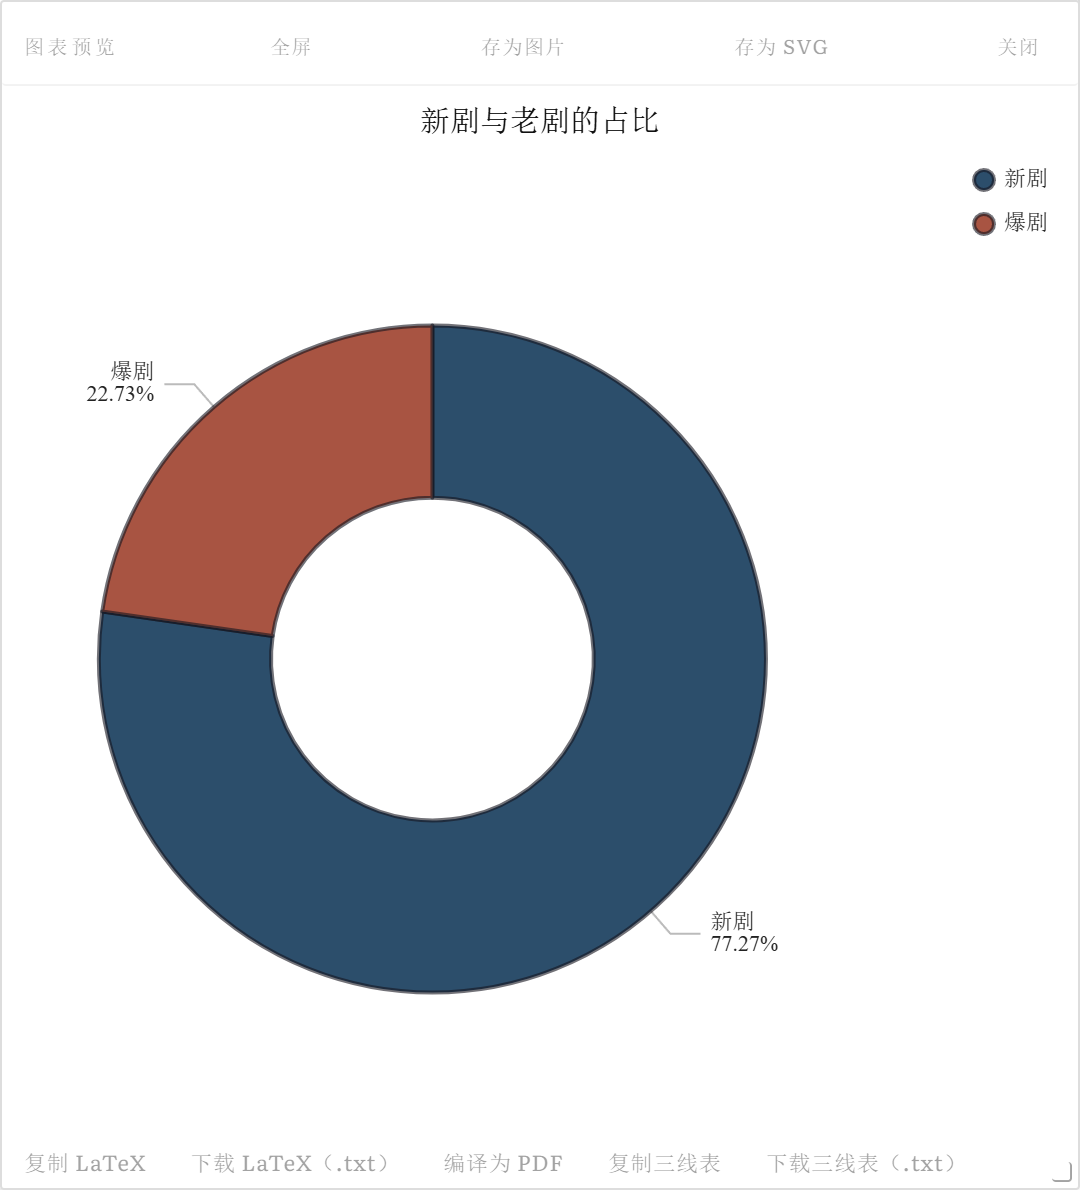
\includegraphics[width=0.84\textwidth]{chart-preview.png}
\caption{图表预览：顶部四个按钮，底部一排 LaTeX 与编译操作}
\label{fig:chart-preview}
\end{figure}

“\texttt{全屏}”把这张图放进一个可拖动、可缩放的浮窗，适合把一页论文大小的图放到最大看细节，也方便直接截图。
窗口顶上同样有存为图片、存为 SVG、关闭。

\begin{figure}[H]\centering
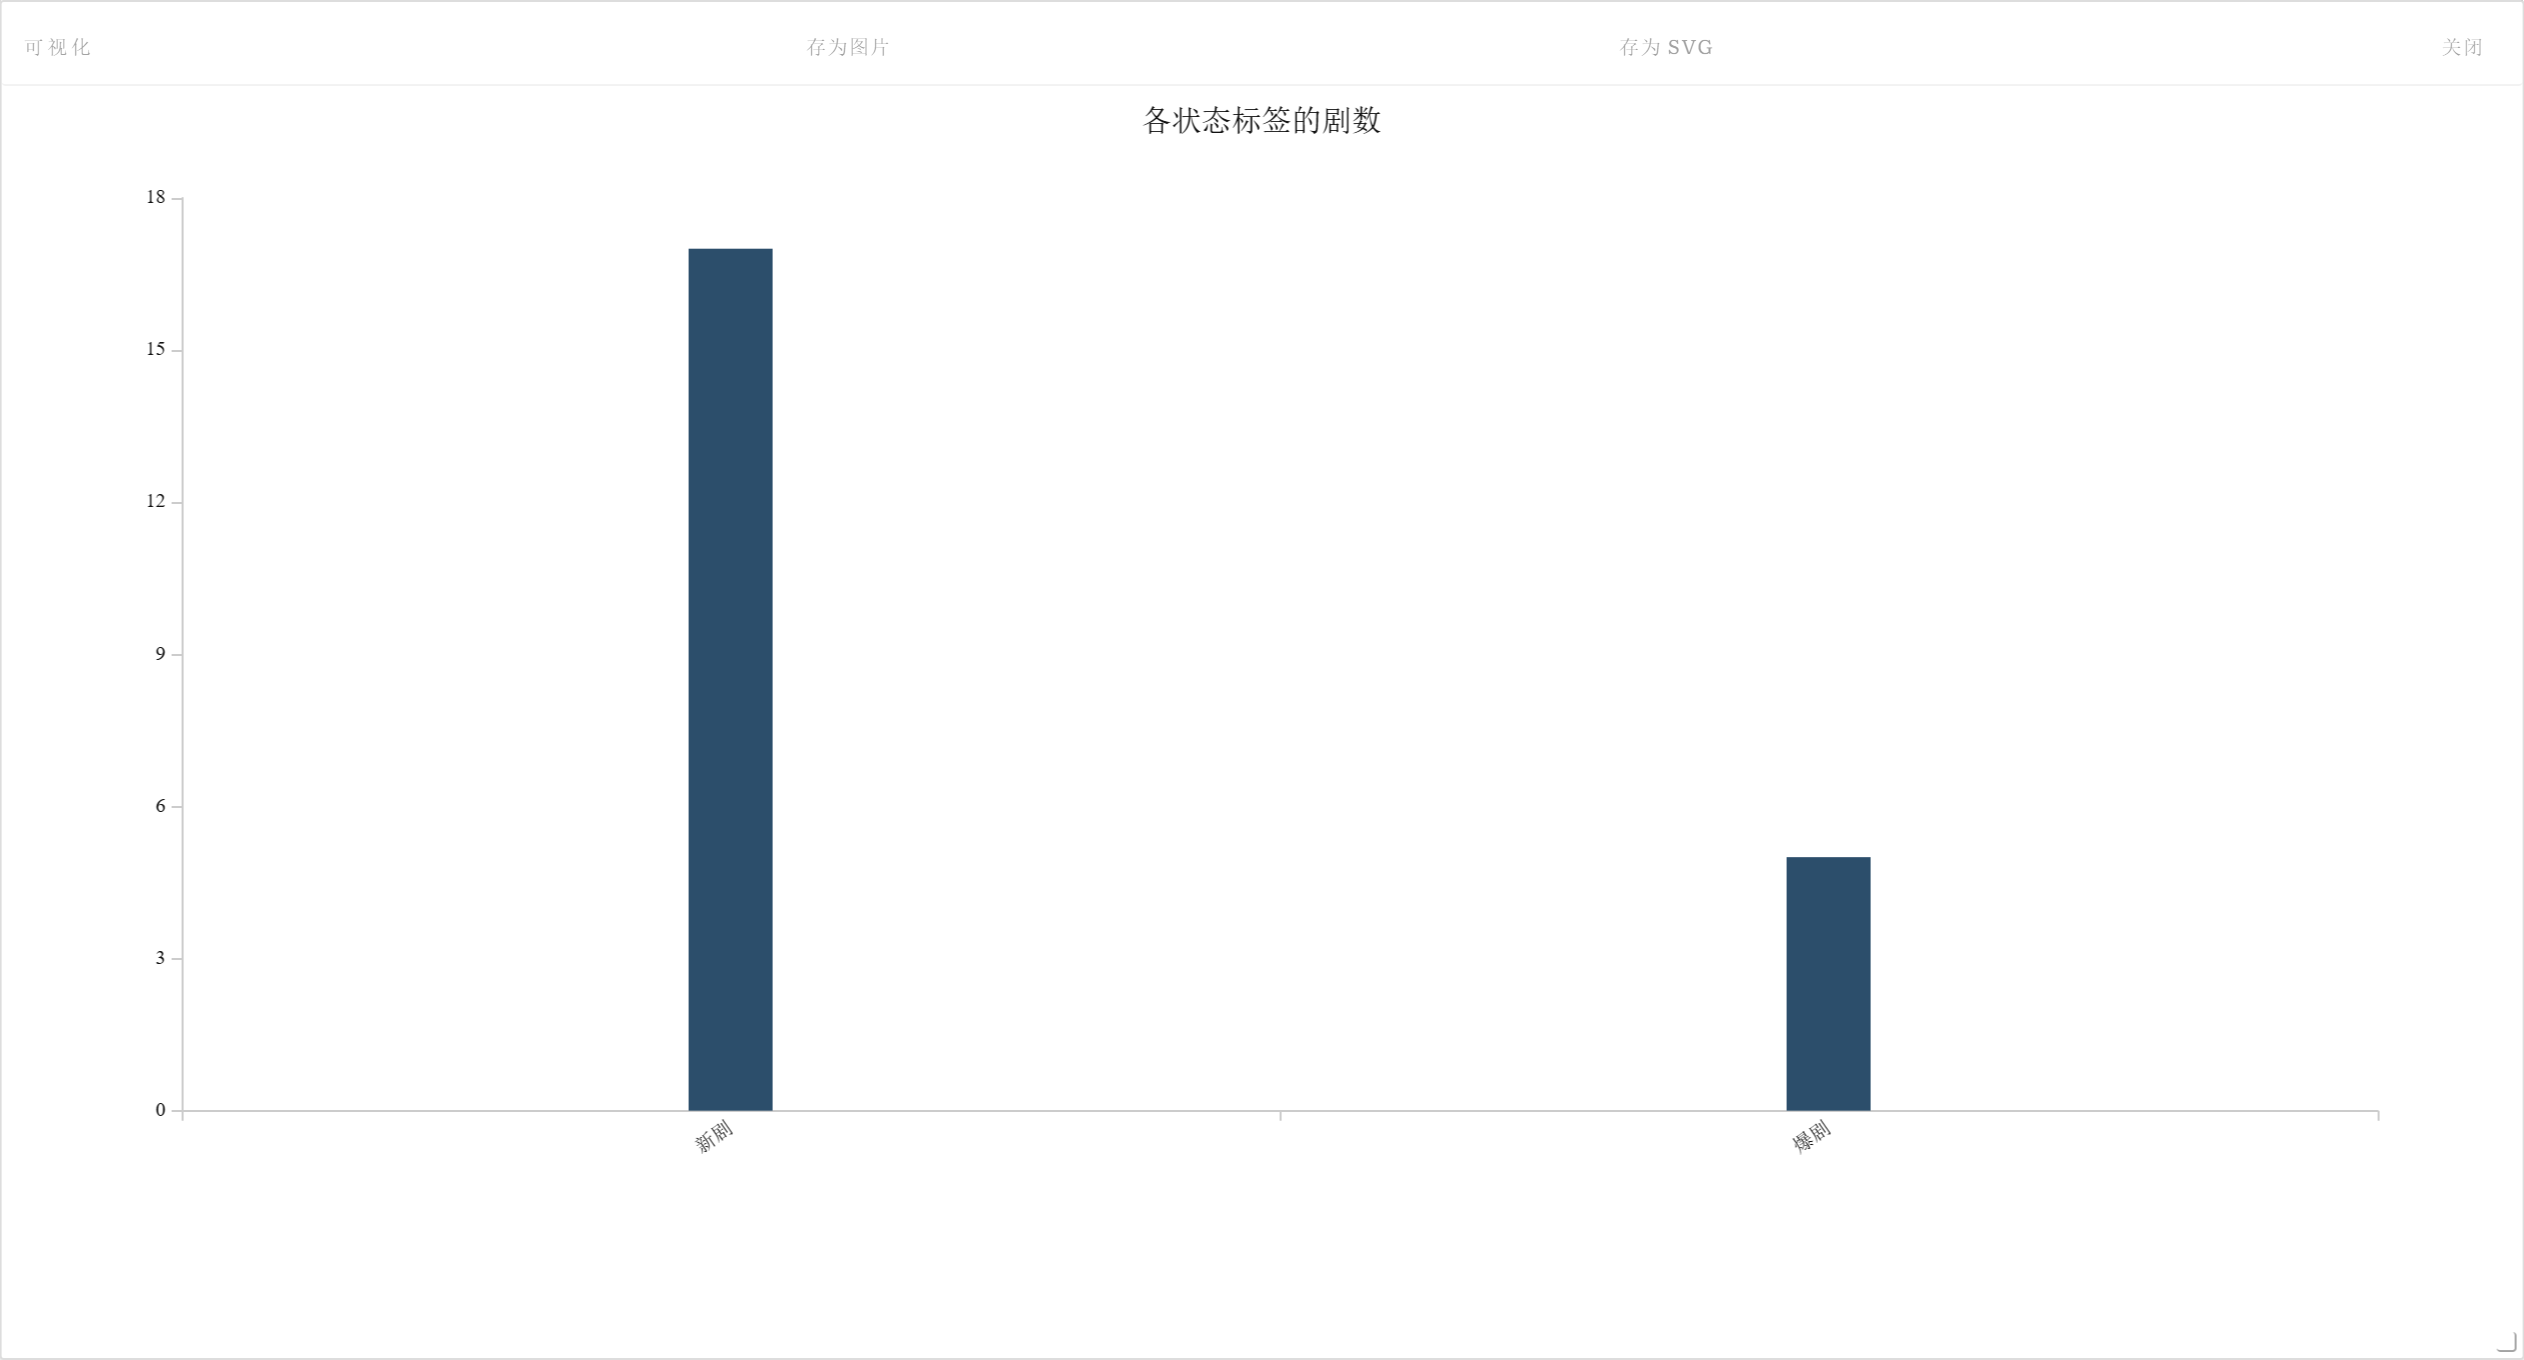
\includegraphics[width=0.96\textwidth]{dashboard-zoom.png}
\caption{从看板点开的全屏图，一个节点一张，可拖动与缩放}
\label{fig:dashboard-zoom}
\end{figure}

菜单条“\texttt{看板}”把画布上所有可视化节点的图拼在一个网格里，一屏看完全部结论。刷新页面会自动回填，
图是数据行的投影，不单独存一份；没有结果的格子写一句先跑一次工作流，是灰字提示，不是报错。

每个格子右上角有“\texttt{全屏}”与“\texttt{存为图片}”，全屏打开的就是上一张图那个浮窗。面板右上角“\texttt{刷新}”重新取数。

\begin{figure}[H]\centering
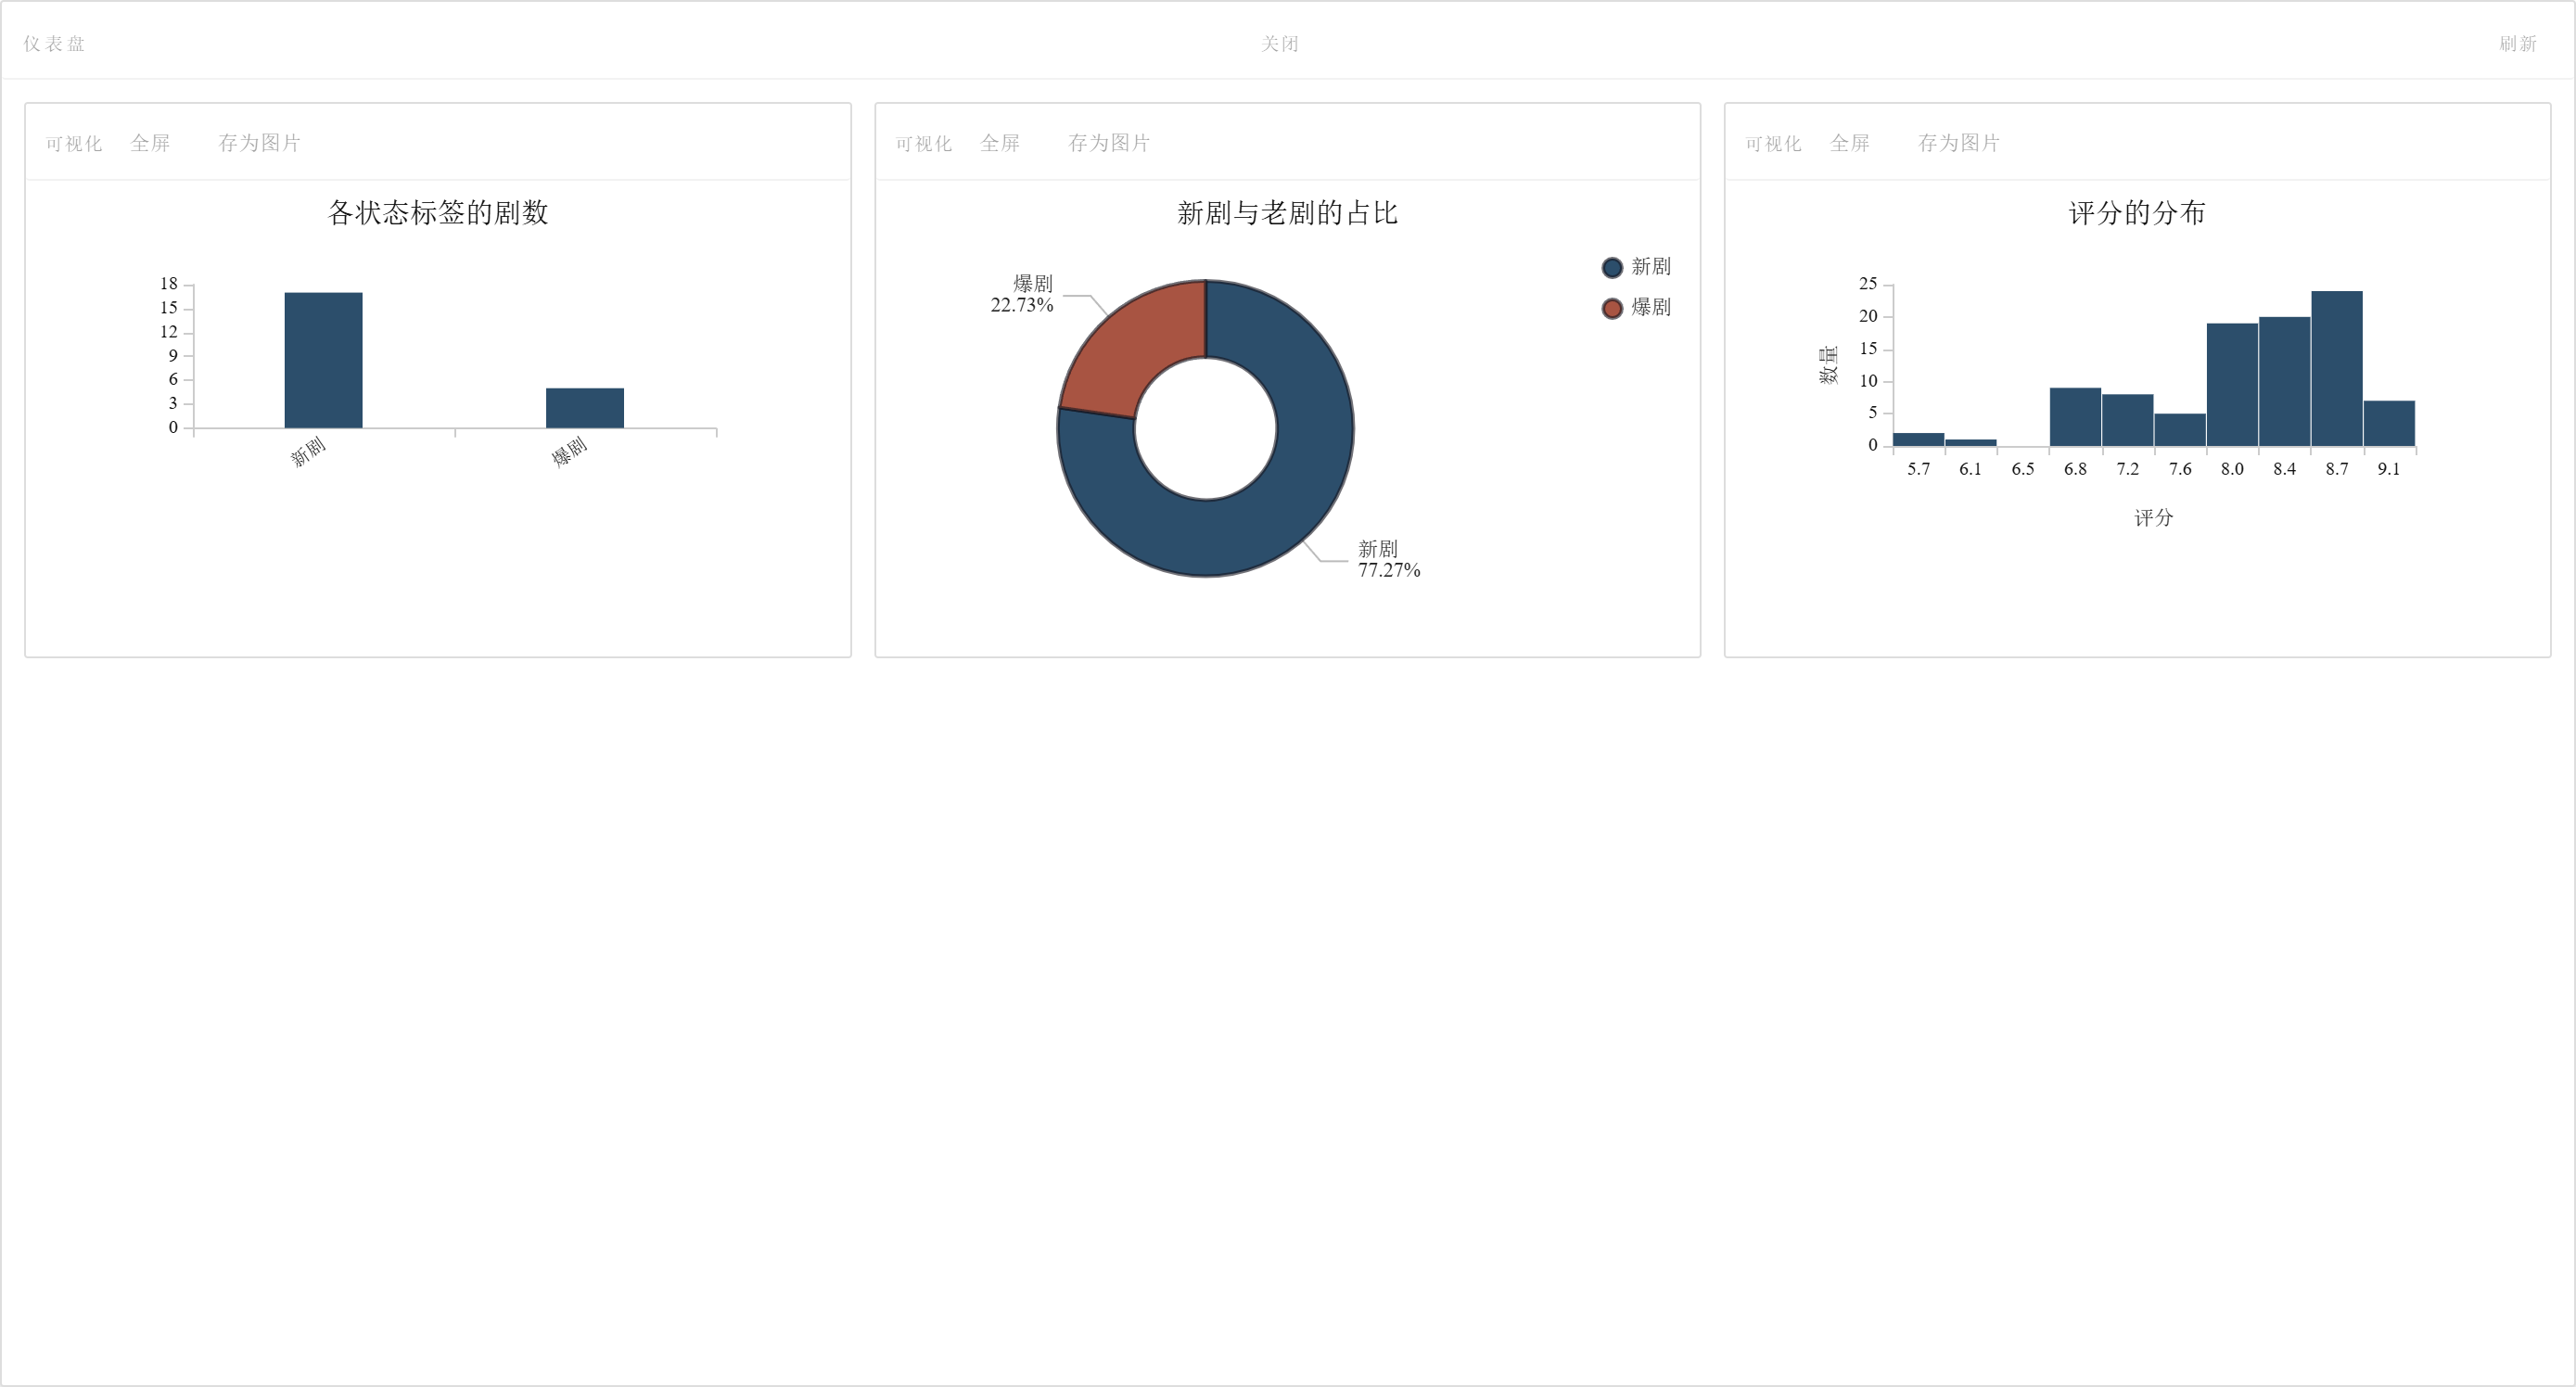
\includegraphics[width=0.98\textwidth]{dashboard.png}
\caption{看板：三个可视化节点并排，每格都能全屏与存图}
\label{fig:dashboard}
\end{figure}

菜单条“\texttt{图表工坊}”是一个内嵌的作图台。可以把任意节点或数据集的整张表交给它自由创作，支持多数据源合并；
自己做好的 PNG 能存回导出目录。适合临时换一种看法，不必为了看一眼而改画布。

\section{报告与执行历史}

工具栏的“\texttt{生成报告}”把一次运行的每张表与服务端渲染的图拼成一个自包含的 HTML，样式与图片都内联，离线能看能打印。
可以附一段模型写的结论，只根据统计数字说话，也可以再打印成 PDF。

“\texttt{历史}”面板按工作流与指标看每次运行的数值走向：情感、倾向、行数三个指标各一条曲线，同一份工作流跑了很多次时，
用它看指标有没有漂移，也能把某次运行的行数与原表对照。

\section{导出与 LaTeX}

\subsection{三种存法}

预览面板和看板每个格子都能把图存成两倍像素的 PNG，或者存成矢量 SVG，文件名就是节点标题，落在导出目录里。
还没有画出来的图不发请求，会提示先预览或者先跑完。数据表则由输出节点存成 CSV、JSON、Excel、文本、HTML、Markdown、Parquet。

\begin{figure}[H]\centering

\includegraphics[width=0.96\textwidth]{exports.png}
\caption{导出产物：文件名、类型、大小、修改时间，每行可下载、删除、复制路径}
\label{fig:exports}
\end{figure}

\subsection{LaTeX 图源与三线表}

每个可视化节点默认生成一份 LaTeX 图源，独立文档，xelatex 直接编译成矢量 PDF，也可以把其中的 figure 部分复制进自己的论文。
它对齐手工精修的观感：仿宋、淡网格、千分位、标签带白底圆角框与引线。另有默认开启的三线表，
表格超过一页时会切成整页的块，续块标上续字，一行不丢。

\subsection{编译节点}

编译节点的上游只能是可视化节点，它把图和表合成一份文档，用本机 xelatex 编成一个 PDF。找不到编译器时只让这一个节点失败并说明缺什么，
不会崩掉整轮；编译失败时读的是日志文件而不是屏幕输出，缺宏包与缺字体各有各的说法。输出节点的格式跟着上游走，
接的是可视化或者编译节点时，下拉里只给 PDF。

\subsection{论文成稿}

报告面板里的“\texttt{论文成稿}”只交运行编号与标题。图和表都从这次运行登记过的 LaTeX 源读回来，
所以成稿里的图与预览里的图不可能是两份。前面附方法段，逐节点写出分析单元与参数；后面附工作流名、运行编号、时间窗与图表数。
它先写 tex 再编译，编译器拒绝时留下的就是那份可以继续排查的源文件，不会留半份 PDF。
